% ========== 3.2 USE CASE ANALYSIS ==========
% Analysis of system use cases and architectural validation

\section{3.2 Use Case Analysis}
\addcontentsline{toc}{section}{3.2 Use Case Analysis}
\label{sec:use-case-analysis}

\lettrine{U}{se case analysis} examines how stakeholders interact with Symphony to accomplish development goals, validating that the architectural design supports real-world workflows. Each use case demonstrates specific system capabilities and identifies the architectural components involved in delivering functionality.

\subsection*{3.2.1 Primary Use Cases}

\textbf{Rapid Application Development:} Developer describes desired functionality in natural language. The Conductor orchestrates multi-model workflow: Enhancer-Prompt expands requirements into technical specifications, Feature model creates structured backlog, Planner designs architecture, Coordinator sequences tasks, Code-Visualizer creates pseudocode, and Editor generates production code. The Artifact Store maintains context across stages while DAG Tracker manages dependencies. This validates the multi-model orchestration approach and artifact-based workflow design.

\textbf{Code Refactoring:} Developer selects code requiring improvement. System employs static analysis to understand structure, orchestrates specialized refactoring models to identify improvements, and generates transformed code with behavior validation. Maintains audit trail for rollback capability. This demonstrates text editor integration, AI model specialization, and safety mechanisms through human oversight.

\textbf{Collaborative Development:} Multiple team members work on shared codebase. System tracks dependencies between code sections, alerts on potential conflicts, provides shared Artifact Store access, and enables workflow template sharing. This validates distributed artifact synchronization, conflict detection mechanisms, and multi-user support design.

\textbf{Learning and Skill Development:} Developer encounters unfamiliar concepts and requests explanation. System analyzes code context, provides tailored explanations relating new concepts to familiar patterns, generates example code, and adapts based on developer responses. This demonstrates context-aware AI models and adaptive assistance capabilities.

\textbf{Debugging and Problem Resolution:} Developer encounters errors or unexpected behavior. System analyzes error messages, examines execution paths, identifies likely causes, suggests debugging strategies, and provides solutions with explanations. This validates integration with error reporting, specialized diagnostic models, and context tracking throughout development lifecycle.


These use cases provide concrete validation criteria for architectural decisions and establish interaction patterns guiding user interface design. Each component can be evaluated based on how effectively it supports real-world development scenarios, ensuring Symphony's architecture directly serves its intended purpose.
% \clearpage
\subsection*{3.2.2 System Use Case Diagram}

The use case diagram provides a comprehensive visual representation of Symphony's functionality and actor interactions. the diverse use cases supported by the system, demonstrating its flexibility and breadth of functionality across different development scenarios as illustrated in Figure 3.1.

\begin{figure}[H]
\centering
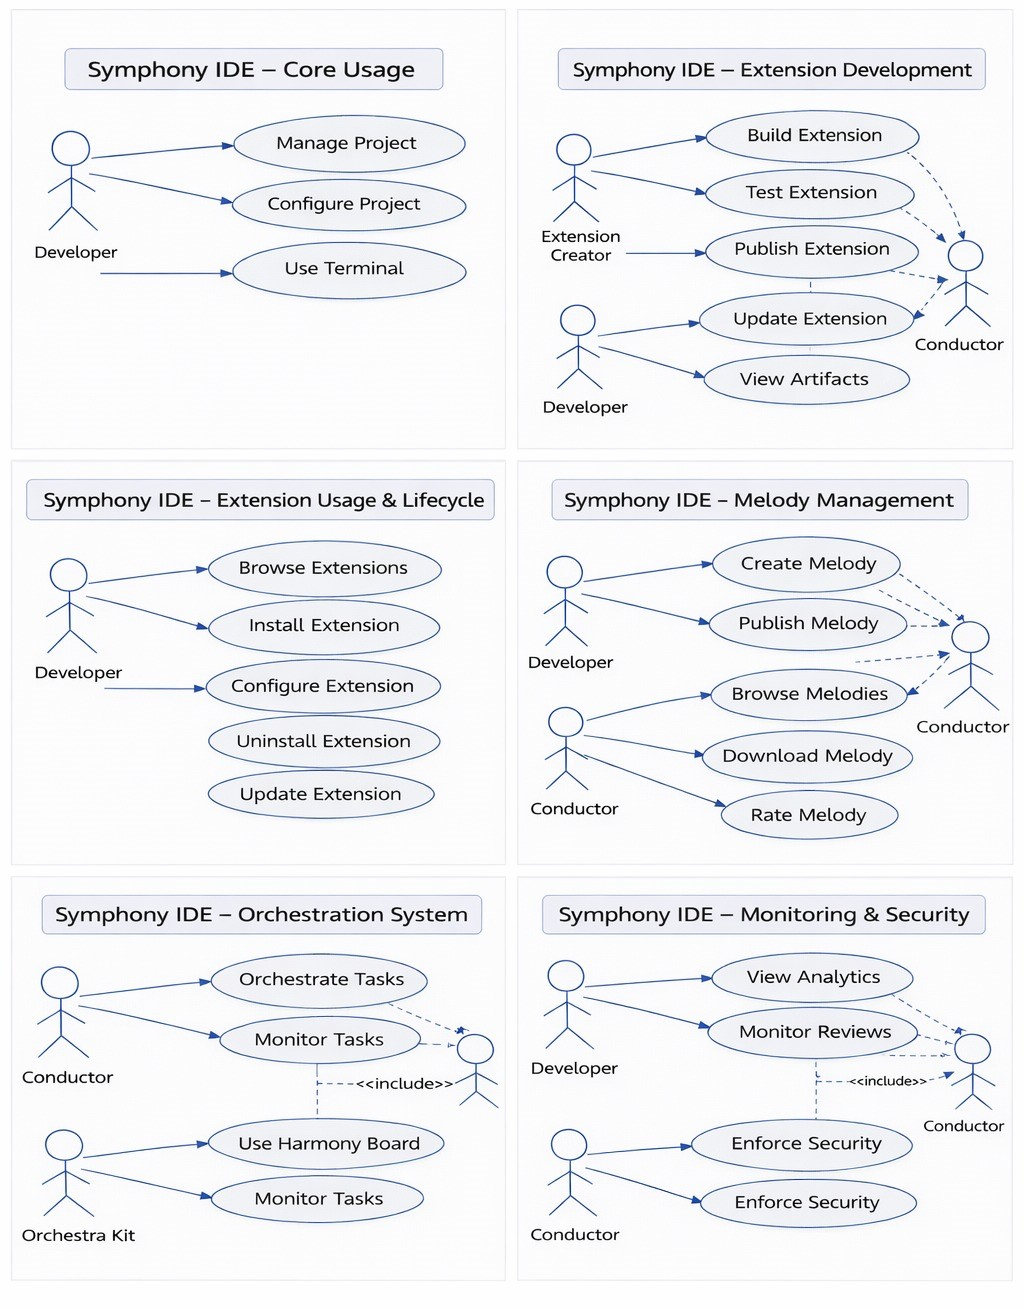
\includegraphics[width=0.85\textwidth]{images/diagrams/usecase.jpeg}
\caption{System Use Cases Diagram}
\label{fig:3.5-usecases}
\end{figure}


